\begin{blocksection}
\question Imagine a trie storing the words "bee", "beekeeper", and "zoo". In a normal trie, we would just have nodes for each character, despite character repeats within each word (2 e's in bee, 2 o's in zoo.
\begin{enumerate}
    \item How could you modify the trie such that repeating characters don't make duplicate nodes in the trie?
    \item Draw out what your new memory efficient Trie would look like if we inserted the words "bee", "beekeeper", "buzz", and "brrrrrr"
    \item When do you expect this Memory Efficient form of trie to use less memory than regular ones? When would it use more?
\end{enumerate}

\begin{solution}[1in]
\begin{enumerate}
    \item Add a field in the Trie Node to keep track of how many repeats of the character there are
    \item It should look something like this 
        \newline 
        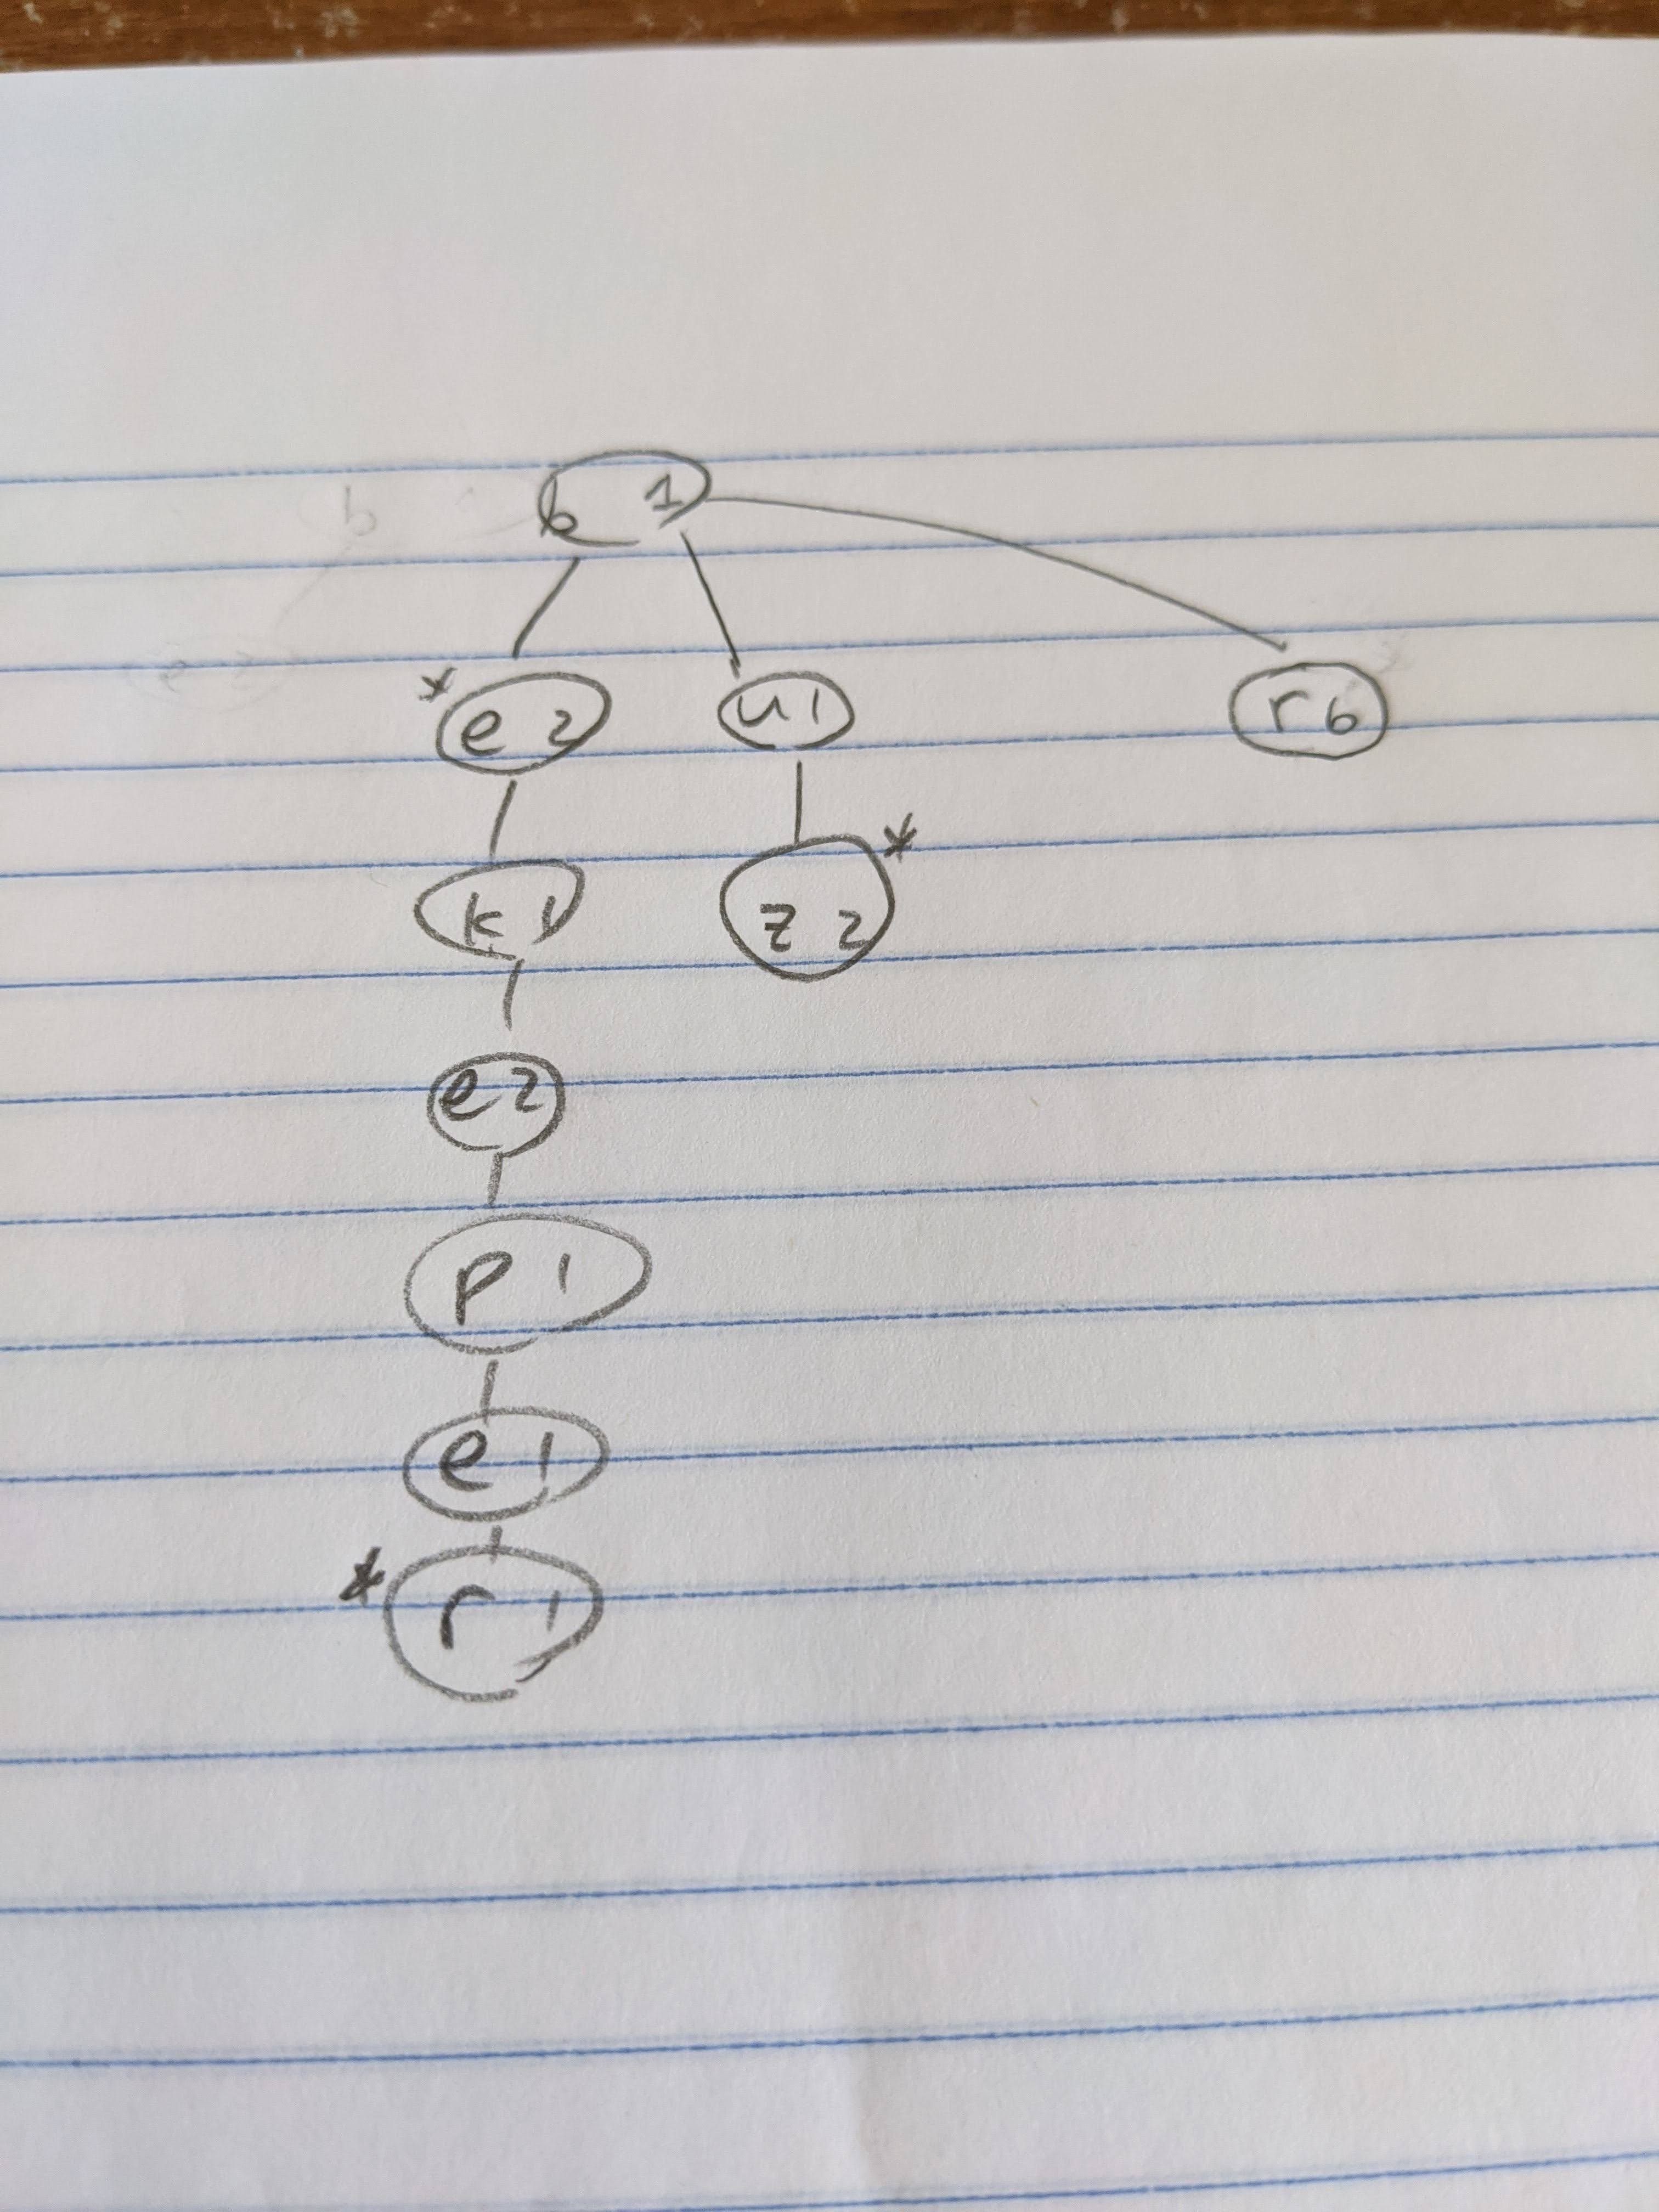
\includegraphics[scale=0.1]{topics/trees/tries/medium/trie.jpg}
    \item If there's lots of repeated characters, it should save some space. If there's very few, it would take more space because it takes memory to keep track of a repeat count in each node.
\end{enumerate}
\end{solution}

\end{blocksection}